    \tikzset{every picture/.style={line width=0.75pt}} %set default line width to 0.75pt        
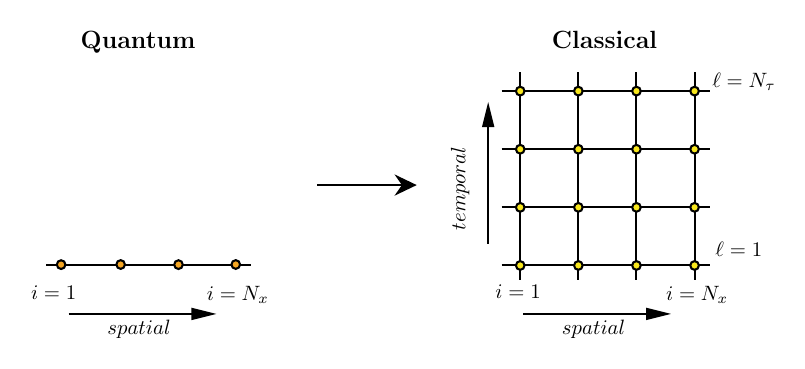
\begin{tikzpicture}[x=0.75pt,y=0.75pt,yscale=-1,xscale=1]
%uncomment if require: \path (0,300); %set diagram left start at 0, and has height of 300

%Straight Lines [id:da49066745050628113] 
\draw    (231.44,120.19) -- (231.44,54.04) ;
\draw [shift={(231.44,52.04)}, rotate = 90] [fill={rgb, 255:red, 0; green, 0; blue, 0 }  ][line width=0.08]  [draw opacity=0] (12,-3) -- (0,0) -- (12,3) -- cycle    ;
%Shape: Grid [id:dp6349220485420457] 
\draw  [draw opacity=0] (237.87,37.73) -- (338.47,37.73) -- (338.47,137.93) -- (237.87,137.93) -- cycle ; \draw   (246.87,37.73) -- (246.87,137.93)(274.87,37.73) -- (274.87,137.93)(302.87,37.73) -- (302.87,137.93)(330.87,37.73) -- (330.87,137.93) ; \draw   (237.87,46.73) -- (338.47,46.73)(237.87,74.73) -- (338.47,74.73)(237.87,102.73) -- (338.47,102.73)(237.87,130.73) -- (338.47,130.73) ; \draw    ;
%Shape: Ellipse [id:dp5284378504134954] 
\draw  [color={rgb, 255:red, 0; green, 0; blue, 0 }  ,draw opacity=1 ][fill={rgb, 255:red, 248; green, 231; blue, 28 }  ,fill opacity=1 ] (244.8,130.73) .. controls (244.8,129.57) and (245.72,128.63) .. (246.87,128.63) .. controls (248.01,128.63) and (248.94,129.57) .. (248.94,130.73) .. controls (248.94,131.9) and (248.01,132.84) .. (246.87,132.84) .. controls (245.72,132.84) and (244.8,131.9) .. (244.8,130.73) -- cycle ;
%Shape: Ellipse [id:dp6215624518257619] 
\draw  [color={rgb, 255:red, 0; green, 0; blue, 0 }  ,draw opacity=1 ][fill={rgb, 255:red, 248; green, 231; blue, 28 }  ,fill opacity=1 ] (272.8,130.73) .. controls (272.8,129.57) and (273.72,128.63) .. (274.87,128.63) .. controls (276.01,128.63) and (276.94,129.57) .. (276.94,130.73) .. controls (276.94,131.9) and (276.01,132.84) .. (274.87,132.84) .. controls (273.72,132.84) and (272.8,131.9) .. (272.8,130.73) -- cycle ;
%Shape: Ellipse [id:dp9063228977247924] 
\draw  [color={rgb, 255:red, 0; green, 0; blue, 0 }  ,draw opacity=1 ][fill={rgb, 255:red, 248; green, 231; blue, 28 }  ,fill opacity=1 ] (300.8,130.73) .. controls (300.8,129.57) and (301.72,128.63) .. (302.87,128.63) .. controls (304.01,128.63) and (304.94,129.57) .. (304.94,130.73) .. controls (304.94,131.9) and (304.01,132.84) .. (302.87,132.84) .. controls (301.72,132.84) and (300.8,131.9) .. (300.8,130.73) -- cycle ;
%Shape: Ellipse [id:dp08954478437422653] 
\draw  [color={rgb, 255:red, 0; green, 0; blue, 0 }  ,draw opacity=1 ][fill={rgb, 255:red, 248; green, 231; blue, 28 }  ,fill opacity=1 ] (328.8,130.73) .. controls (328.8,129.57) and (329.72,128.63) .. (330.87,128.63) .. controls (332.01,128.63) and (332.94,129.57) .. (332.94,130.73) .. controls (332.94,131.9) and (332.01,132.84) .. (330.87,132.84) .. controls (329.72,132.84) and (328.8,131.9) .. (328.8,130.73) -- cycle ;
%Shape: Ellipse [id:dp33764670524957285] 
\draw  [color={rgb, 255:red, 0; green, 0; blue, 0 }  ,draw opacity=1 ][fill={rgb, 255:red, 248; green, 231; blue, 28 }  ,fill opacity=1 ] (328.8,102.73) .. controls (328.8,101.57) and (329.72,100.63) .. (330.87,100.63) .. controls (332.01,100.63) and (332.94,101.57) .. (332.94,102.73) .. controls (332.94,103.9) and (332.01,104.84) .. (330.87,104.84) .. controls (329.72,104.84) and (328.8,103.9) .. (328.8,102.73) -- cycle ;
%Shape: Ellipse [id:dp41409094313145167] 
\draw  [color={rgb, 255:red, 0; green, 0; blue, 0 }  ,draw opacity=1 ][fill={rgb, 255:red, 248; green, 231; blue, 28 }  ,fill opacity=1 ] (300.8,102.73) .. controls (300.8,101.57) and (301.72,100.63) .. (302.87,100.63) .. controls (304.01,100.63) and (304.94,101.57) .. (304.94,102.73) .. controls (304.94,103.9) and (304.01,104.84) .. (302.87,104.84) .. controls (301.72,104.84) and (300.8,103.9) .. (300.8,102.73) -- cycle ;
%Shape: Ellipse [id:dp6015308484706063] 
\draw  [color={rgb, 255:red, 0; green, 0; blue, 0 }  ,draw opacity=1 ][fill={rgb, 255:red, 248; green, 231; blue, 28 }  ,fill opacity=1 ] (272.8,102.73) .. controls (272.8,101.57) and (273.72,100.63) .. (274.87,100.63) .. controls (276.01,100.63) and (276.94,101.57) .. (276.94,102.73) .. controls (276.94,103.9) and (276.01,104.84) .. (274.87,104.84) .. controls (273.72,104.84) and (272.8,103.9) .. (272.8,102.73) -- cycle ;
%Shape: Ellipse [id:dp931775421174188] 
\draw  [color={rgb, 255:red, 0; green, 0; blue, 0 }  ,draw opacity=1 ][fill={rgb, 255:red, 248; green, 231; blue, 28 }  ,fill opacity=1 ] (244.8,102.73) .. controls (244.8,101.57) and (245.72,100.63) .. (246.87,100.63) .. controls (248.01,100.63) and (248.94,101.57) .. (248.94,102.73) .. controls (248.94,103.9) and (248.01,104.84) .. (246.87,104.84) .. controls (245.72,104.84) and (244.8,103.9) .. (244.8,102.73) -- cycle ;
%Shape: Ellipse [id:dp9347505046448723] 
\draw  [color={rgb, 255:red, 0; green, 0; blue, 0 }  ,draw opacity=1 ][fill={rgb, 255:red, 248; green, 231; blue, 28 }  ,fill opacity=1 ] (244.8,74.73) .. controls (244.8,73.57) and (245.72,72.63) .. (246.87,72.63) .. controls (248.01,72.63) and (248.94,73.57) .. (248.94,74.73) .. controls (248.94,75.9) and (248.01,76.84) .. (246.87,76.84) .. controls (245.72,76.84) and (244.8,75.9) .. (244.8,74.73) -- cycle ;
%Shape: Ellipse [id:dp914231137007502] 
\draw  [color={rgb, 255:red, 0; green, 0; blue, 0 }  ,draw opacity=1 ][fill={rgb, 255:red, 248; green, 231; blue, 28 }  ,fill opacity=1 ] (272.8,74.73) .. controls (272.8,73.57) and (273.72,72.63) .. (274.87,72.63) .. controls (276.01,72.63) and (276.94,73.57) .. (276.94,74.73) .. controls (276.94,75.9) and (276.01,76.84) .. (274.87,76.84) .. controls (273.72,76.84) and (272.8,75.9) .. (272.8,74.73) -- cycle ;
%Shape: Ellipse [id:dp3096522809403266] 
\draw  [color={rgb, 255:red, 0; green, 0; blue, 0 }  ,draw opacity=1 ][fill={rgb, 255:red, 248; green, 231; blue, 28 }  ,fill opacity=1 ] (300.8,74.73) .. controls (300.8,73.57) and (301.72,72.63) .. (302.87,72.63) .. controls (304.01,72.63) and (304.94,73.57) .. (304.94,74.73) .. controls (304.94,75.9) and (304.01,76.84) .. (302.87,76.84) .. controls (301.72,76.84) and (300.8,75.9) .. (300.8,74.73) -- cycle ;
%Shape: Ellipse [id:dp06969323865861776] 
\draw  [color={rgb, 255:red, 0; green, 0; blue, 0 }  ,draw opacity=1 ][fill={rgb, 255:red, 248; green, 231; blue, 28 }  ,fill opacity=1 ] (328.8,74.73) .. controls (328.8,73.57) and (329.72,72.63) .. (330.87,72.63) .. controls (332.01,72.63) and (332.94,73.57) .. (332.94,74.73) .. controls (332.94,75.9) and (332.01,76.84) .. (330.87,76.84) .. controls (329.72,76.84) and (328.8,75.9) .. (328.8,74.73) -- cycle ;
%Shape: Ellipse [id:dp25713744690136875] 
\draw  [color={rgb, 255:red, 0; green, 0; blue, 0 }  ,draw opacity=1 ][fill={rgb, 255:red, 248; green, 231; blue, 28 }  ,fill opacity=1 ] (328.8,46.73) .. controls (328.8,45.57) and (329.72,44.63) .. (330.87,44.63) .. controls (332.01,44.63) and (332.94,45.57) .. (332.94,46.73) .. controls (332.94,47.9) and (332.01,48.84) .. (330.87,48.84) .. controls (329.72,48.84) and (328.8,47.9) .. (328.8,46.73) -- cycle ;
%Shape: Ellipse [id:dp4907206909327364] 
\draw  [color={rgb, 255:red, 0; green, 0; blue, 0 }  ,draw opacity=1 ][fill={rgb, 255:red, 248; green, 231; blue, 28 }  ,fill opacity=1 ] (300.8,46.73) .. controls (300.8,45.57) and (301.72,44.63) .. (302.87,44.63) .. controls (304.01,44.63) and (304.94,45.57) .. (304.94,46.73) .. controls (304.94,47.9) and (304.01,48.84) .. (302.87,48.84) .. controls (301.72,48.84) and (300.8,47.9) .. (300.8,46.73) -- cycle ;
%Shape: Ellipse [id:dp29947202378858284] 
\draw  [color={rgb, 255:red, 0; green, 0; blue, 0 }  ,draw opacity=1 ][fill={rgb, 255:red, 248; green, 231; blue, 28 }  ,fill opacity=1 ] (272.8,46.73) .. controls (272.8,45.57) and (273.72,44.63) .. (274.87,44.63) .. controls (276.01,44.63) and (276.94,45.57) .. (276.94,46.73) .. controls (276.94,47.9) and (276.01,48.84) .. (274.87,48.84) .. controls (273.72,48.84) and (272.8,47.9) .. (272.8,46.73) -- cycle ;
%Shape: Ellipse [id:dp4185338076770435] 
\draw  [color={rgb, 255:red, 0; green, 0; blue, 0 }  ,draw opacity=1 ][fill={rgb, 255:red, 248; green, 231; blue, 28 }  ,fill opacity=1 ] (244.8,46.73) .. controls (244.8,45.57) and (245.72,44.63) .. (246.87,44.63) .. controls (248.01,44.63) and (248.94,45.57) .. (248.94,46.73) .. controls (248.94,47.9) and (248.01,48.84) .. (246.87,48.84) .. controls (245.72,48.84) and (244.8,47.9) .. (244.8,46.73) -- cycle ;
%Straight Lines [id:da43115254468649855] 
\draw    (248.33,154.08) -- (317.49,154.08) ;
\draw [shift={(319.49,154.08)}, rotate = 180] [fill={rgb, 255:red, 0; green, 0; blue, 0 }  ][line width=0.08]  [draw opacity=0] (12,-3) -- (0,0) -- (12,3) -- cycle    ;
%Straight Lines [id:da5861440787349572] 
\draw    (18.52,130.33) -- (117.06,130.33) ;
%Shape: Ellipse [id:dp9617050388696362] 
\draw  [color={rgb, 255:red, 0; green, 0; blue, 0 }  ,draw opacity=1 ][fill={rgb, 255:red, 245; green, 166; blue, 35 }  ,fill opacity=1 ] (23.6,130.33) .. controls (23.6,129.17) and (24.52,128.23) .. (25.67,128.23) .. controls (26.81,128.23) and (27.74,129.17) .. (27.74,130.33) .. controls (27.74,131.5) and (26.81,132.44) .. (25.67,132.44) .. controls (24.52,132.44) and (23.6,131.5) .. (23.6,130.33) -- cycle ;
%Shape: Ellipse [id:dp24776284141212535] 
\draw  [color={rgb, 255:red, 0; green, 0; blue, 0 }  ,draw opacity=1 ][fill={rgb, 255:red, 245; green, 166; blue, 35 }  ,fill opacity=1 ] (52.29,130.28) .. controls (52.29,129.12) and (53.21,128.17) .. (54.36,128.17) .. controls (55.5,128.17) and (56.42,129.12) .. (56.42,130.28) .. controls (56.42,131.44) and (55.5,132.38) .. (54.36,132.38) .. controls (53.21,132.38) and (52.29,131.44) .. (52.29,130.28) -- cycle ;
%Shape: Ellipse [id:dp3996487654461587] 
\draw  [color={rgb, 255:red, 0; green, 0; blue, 0 }  ,draw opacity=1 ][fill={rgb, 255:red, 245; green, 166; blue, 35 }  ,fill opacity=1 ] (80.15,130.33) .. controls (80.15,129.17) and (81.07,128.23) .. (82.22,128.23) .. controls (83.36,128.23) and (84.29,129.17) .. (84.29,130.33) .. controls (84.29,131.5) and (83.36,132.44) .. (82.22,132.44) .. controls (81.07,132.44) and (80.15,131.5) .. (80.15,130.33) -- cycle ;
%Shape: Ellipse [id:dp253376514870602] 
\draw  [color={rgb, 255:red, 0; green, 0; blue, 0 }  ,draw opacity=1 ][fill={rgb, 255:red, 245; green, 166; blue, 35 }  ,fill opacity=1 ] (107.74,130.28) .. controls (107.74,129.12) and (108.67,128.17) .. (109.81,128.17) .. controls (110.95,128.17) and (111.88,129.12) .. (111.88,130.28) .. controls (111.88,131.44) and (110.95,132.38) .. (109.81,132.38) .. controls (108.67,132.38) and (107.74,131.44) .. (107.74,130.28) -- cycle ;
%Straight Lines [id:da6189404107389695] 
\draw    (149,92) -- (194,92) ;
\draw [shift={(197,92)}, rotate = 180] [fill={rgb, 255:red, 0; green, 0; blue, 0 }  ][line width=0.08]  [draw opacity=0] (10.72,-5.15) -- (0,0) -- (10.72,5.15) -- (7.12,0) -- cycle    ;
%Straight Lines [id:da8320203387459979] 
\draw    (29.33,154.08) -- (98.49,154.08) ;
\draw [shift={(100.49,154.08)}, rotate = 180] [fill={rgb, 255:red, 0; green, 0; blue, 0 }  ][line width=0.08]  [draw opacity=0] (12,-3) -- (0,0) -- (12,3) -- cycle    ;

% Text Node
\draw (212.32,114.83) node [anchor=north west][inner sep=0.75pt]  [rotate=-270,xscale=0.75,yscale=0.75]  {$\text{temporal}$};
% Text Node
\draw (265.82,156.16) node [anchor=north west][inner sep=0.75pt]  [xscale=0.75,yscale=0.75]  {$\text{spatial}$};
% Text Node
\draw (233.82,138.71) node [anchor=north west][inner sep=0.75pt]  [xscale=0.75,yscale=0.75]  {$i=1$};
% Text Node
\draw (316.04,139.6) node [anchor=north west][inner sep=0.75pt]  [xscale=0.75,yscale=0.75]  {$i=N_x$};
% Text Node
\draw (339.82,118.27) node [anchor=north west][inner sep=0.75pt]  [xscale=0.75,yscale=0.75]  {$\ell =1$};
% Text Node
\draw (338.27,36.93) node [anchor=north west][inner sep=0.75pt]  [xscale=0.75,yscale=0.75]  {$\ell =N_\tau$};
% Text Node
\draw (10.06,139.62) node [anchor=north west][inner sep=0.75pt]  [xscale=0.75,yscale=0.75]  {$i=1$};
% Text Node
\draw (94.79,139.62) node [anchor=north west][inner sep=0.75pt]  [xscale=0.75,yscale=0.75]  {$i=N_x$};
% Text Node
\draw (34,16.67) node [anchor=north west][inner sep=0.75pt]  [font=\large,xscale=0.75,yscale=0.75] [align=left] {\textbf{Quantum}};
% Text Node
\draw (261,16.67) node [anchor=north west][inner sep=0.75pt]  [font=\large,xscale=0.75,yscale=0.75] [align=left] {\textbf{Classical}};
% Text Node
\draw (46.82,156.16) node [anchor=north west][inner sep=0.75pt]  [xscale=0.75,yscale=0.75]  {$\text{spatial}$};


\end{tikzpicture}